\documentclass[tikz,border=3.14mm]{standalone}
\usetikzlibrary{arrows.meta, positioning}

\begin{document}
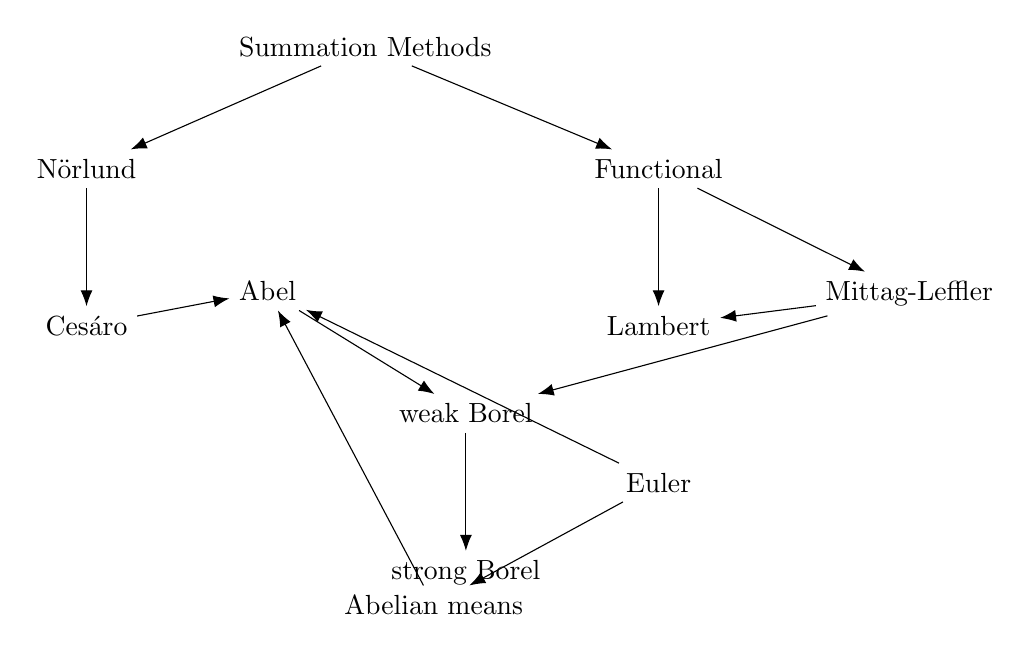
\begin{tikzpicture}[node distance=1.5cm, auto,>={Latex[scale=1.2]}]
    \node[align=center] (sum) {Summation Methods};
    \node[align=center, below left=of sum] (nor) {Nörlund};
    \node[align=center, below right=of sum] (fun) {Functional};
    
    \node[align=center, below=of nor] (ces) {Cesáro};
    \node[align=center, below right=of nor] (abel) {Abel};
    
    \node[align=center, below=of fun] (lam) {Lambert};
    \node[align=center, below right=of fun] (mit) {Mittag-Leffler};
    
    \node[align=center, below right=of abel] (wb) {weak Borel};
    \node[align=center, below=of wb] (sb) {strong Borel};
    
    \node[align=center, below=of lam] (eul) {Euler};
    
    \node[align=center, below left=of eul] (aca) {Abelian means};
    
    \draw[->] (sum) -- (nor);
    \draw[->] (sum) -- (fun);
    
    \draw[->] (nor) -- (ces);
    \draw[->] (ces) -- (abel);
    
    \draw[->] (eul) -- (abel);
    
    \draw[->] (fun) -- (lam);
    \draw[->] (fun) -- (mit);
    
    \draw[->] (abel) -- (wb);
    \draw[->] (wb) -- (sb);
    
    \draw[->] (mit) -- (lam);
    \draw[->] (mit) -- (wb);
    
    \draw[->] (eul) -- (aca);
    \draw[->] (aca) -- (abel);
\end{tikzpicture}
\end{document}